This section reviews some programming languages and how they provide ``freedom from choice'' in the sense of A. Sangiovani-Vincentelli~\cite{lee2019freedom}.
There is a distinct sense in this is the central question of programming languages in general.
By removing memory management through having no pointer arithmetic and garbage collection, Java frees its users from multiple families of errors that are possible in C.
Rust's ownership types take a different approach, also removing complete families of memory-management based errors, without introducing large performance overheads or unpredictable behavior from the garbage collector.
Elm~\cite{czaplicki_elm}, on the other hand, exposes a functional paradigm with a strong type-system for \acsu{GUI} development of web applications, which eliminates virtually all run-time errors.

These kinds of ``freedom from choice'' are beyond the scope of this thesis, which focuses on \acp{MoC} like those described in Chapter~\ref{chap:mocs}.
In more constraining  \acp{MoC}, like the ones discussed here, the temptation to break away from the semantics might be higher.
An interesting observation and discussion of this phenomenon can be found in~\cite{tasharofi2013scala}.
Not only does it show that developers commonly break away from the semantics if these are not enforced, but also gives multiple explanations why.
This is why we believe \acp{MoC} should not be exposed as a library, but rather as implicit in the semantics of a (full) language.
Here we will briefly survey languages focused on \ac{MoC}-based paradigms.

\subsection{Dataflow, Actors and Discrete Events}
\label{sec:general_dataflow_tools}

Most well-known languages that follow \acp{MoC} like the ones described here are based on the actor model.
Compared to more sophisticated models, the actor model has mostly intuitive semantics.
The Erlang language is a successful example of a language whose semantics are in principle an implementation of the (Hewitt-Agha) actor model.\index{Erlang}
Another example of an actor based language is Rebeca~\cite{sirjani2004formal}, which is primarily a design and specification language used in model checking.\index{Rebeca}
Another prominent example is the CAL actor language~\cite{eker2003cal}.
It has been used to define the \ac{RVC} standard~\cite{bhattacharyya2011overview}.
The \ac{RVC}-CAL compiler\footnote{\url{https://sourceforge.net/projects/orcc/}} is an Eclipse-based compiler for the CAL actor language, which is used to compile the \ac{RVC} reference implementations.\index{\ac{RVC}-CAL}

Ptolemy~II\cite{Ptolemaeus:14:SystemDesign} is another prominent \ac{MoC}-centered programming environment.
In contrast to most of the other frameworks, Ptolemy~II supports a plethora of \ac{MoC}, including most of the models discussed in this thesis. 
Also in contrast to most other frameworks, \acp{MoC} are a central component of Ptolemy~II, which makes them explicit using \emph{directors}\index{Ptolemy~II}.
The framework uses the Java programming language to allow the definition of arbitrary actors, but it also comes with a large library of pre-defined actors.
Figure~\ref{fig:audio_filter_ptolemy} shows an implementation of an audio filter, which while not identical, is semantically similar to our running example described in Chapter~\ref{chap:mapping}.
This implementation uses only pre-defined actors in Ptolemy~II.

\begin{figure}[t]
	\centering
	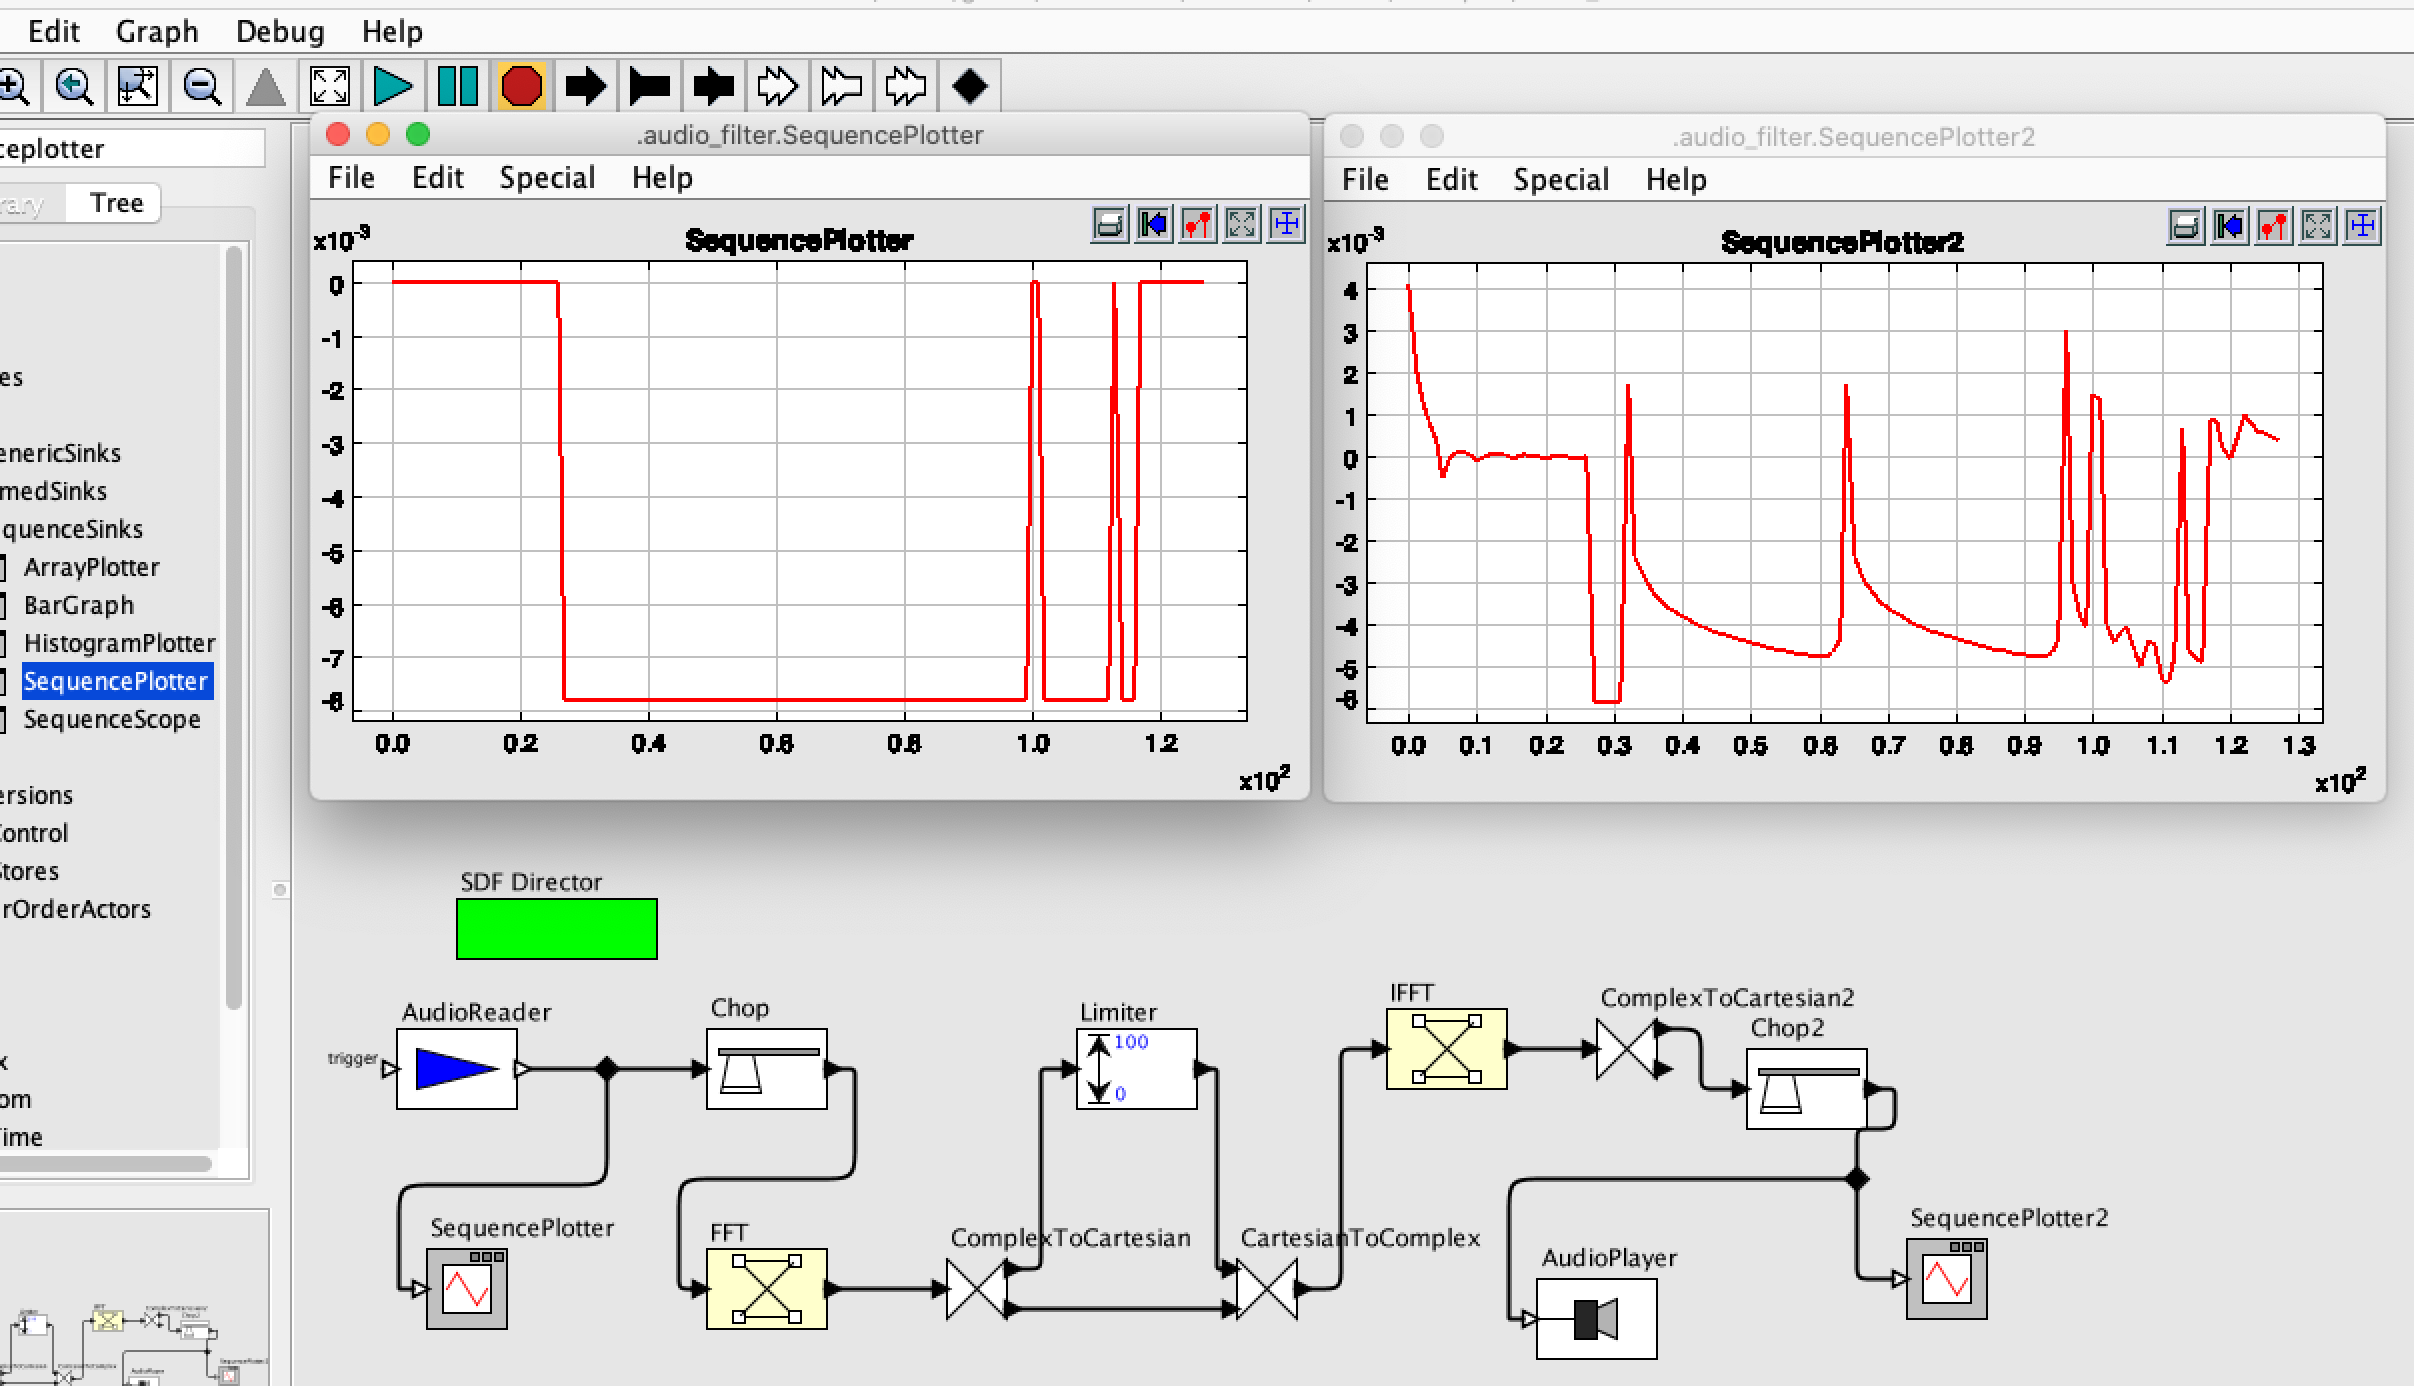
\includegraphics[width=0.9\textwidth]{figures/audio_filter_ptolemy_screenshot.png}
	\caption{An audio filter in \ac{SDF} semantics in Ptolemy II}
	\label{fig:audio_filter_ptolemy}
	%	\vspace{-1mm}
\end{figure}

In the case of discrete-event models, there are many well-established languages which implement them.
The hardware description languages VHDL and Verilog work with discrete-event semantics, since hardware does. 
The SystemC language, well known for discrete event simulations (of hardware), also has discrete event semantics~\cite{semantics_systemc}.
Similarly does the related SpecC language~\cite{specc}.
Finally, more on the software side are the Synchronous languages, like LUSTRE~\cite{lustre} or ESTEREL~\cite{esterel}, which are (complete) programming languages with discrete-event semantics.

The Lingua Franca language~\cite{lohstroh2020language}\footnote{\url{https://github.com/icyphy/lingua-franca}} is  also in the discrete events domain.
Lingua Franca is a complex framework that implements the Reactors model, described in Section~\ref{sec:reactors}.
This novel language is a self-described polyglot \emph{coordination language}, which means that it is not used to define the computation, but rather, to compose reactors written in a different language.
Nothing prevents programmers from ``cheating'' in the code of the reactors and going around the semantics, yet it does enforce them more strongly than a library.
Lingua Franca is a (complete) \ac{DSL} that generates Reactors-based applications in a source-to-source compilation process.
Figure~\ref{fig:audio_filter_lf} shows the Eclipse-based programming environment of Lingua Franca, with an implementation of the audio filter benchmark.
We will not discuss the framework more in detail, as the design and implementation of Lingua Franca is not part of the contribution of this thesis.

\begin{figure}[t]
	\centering
	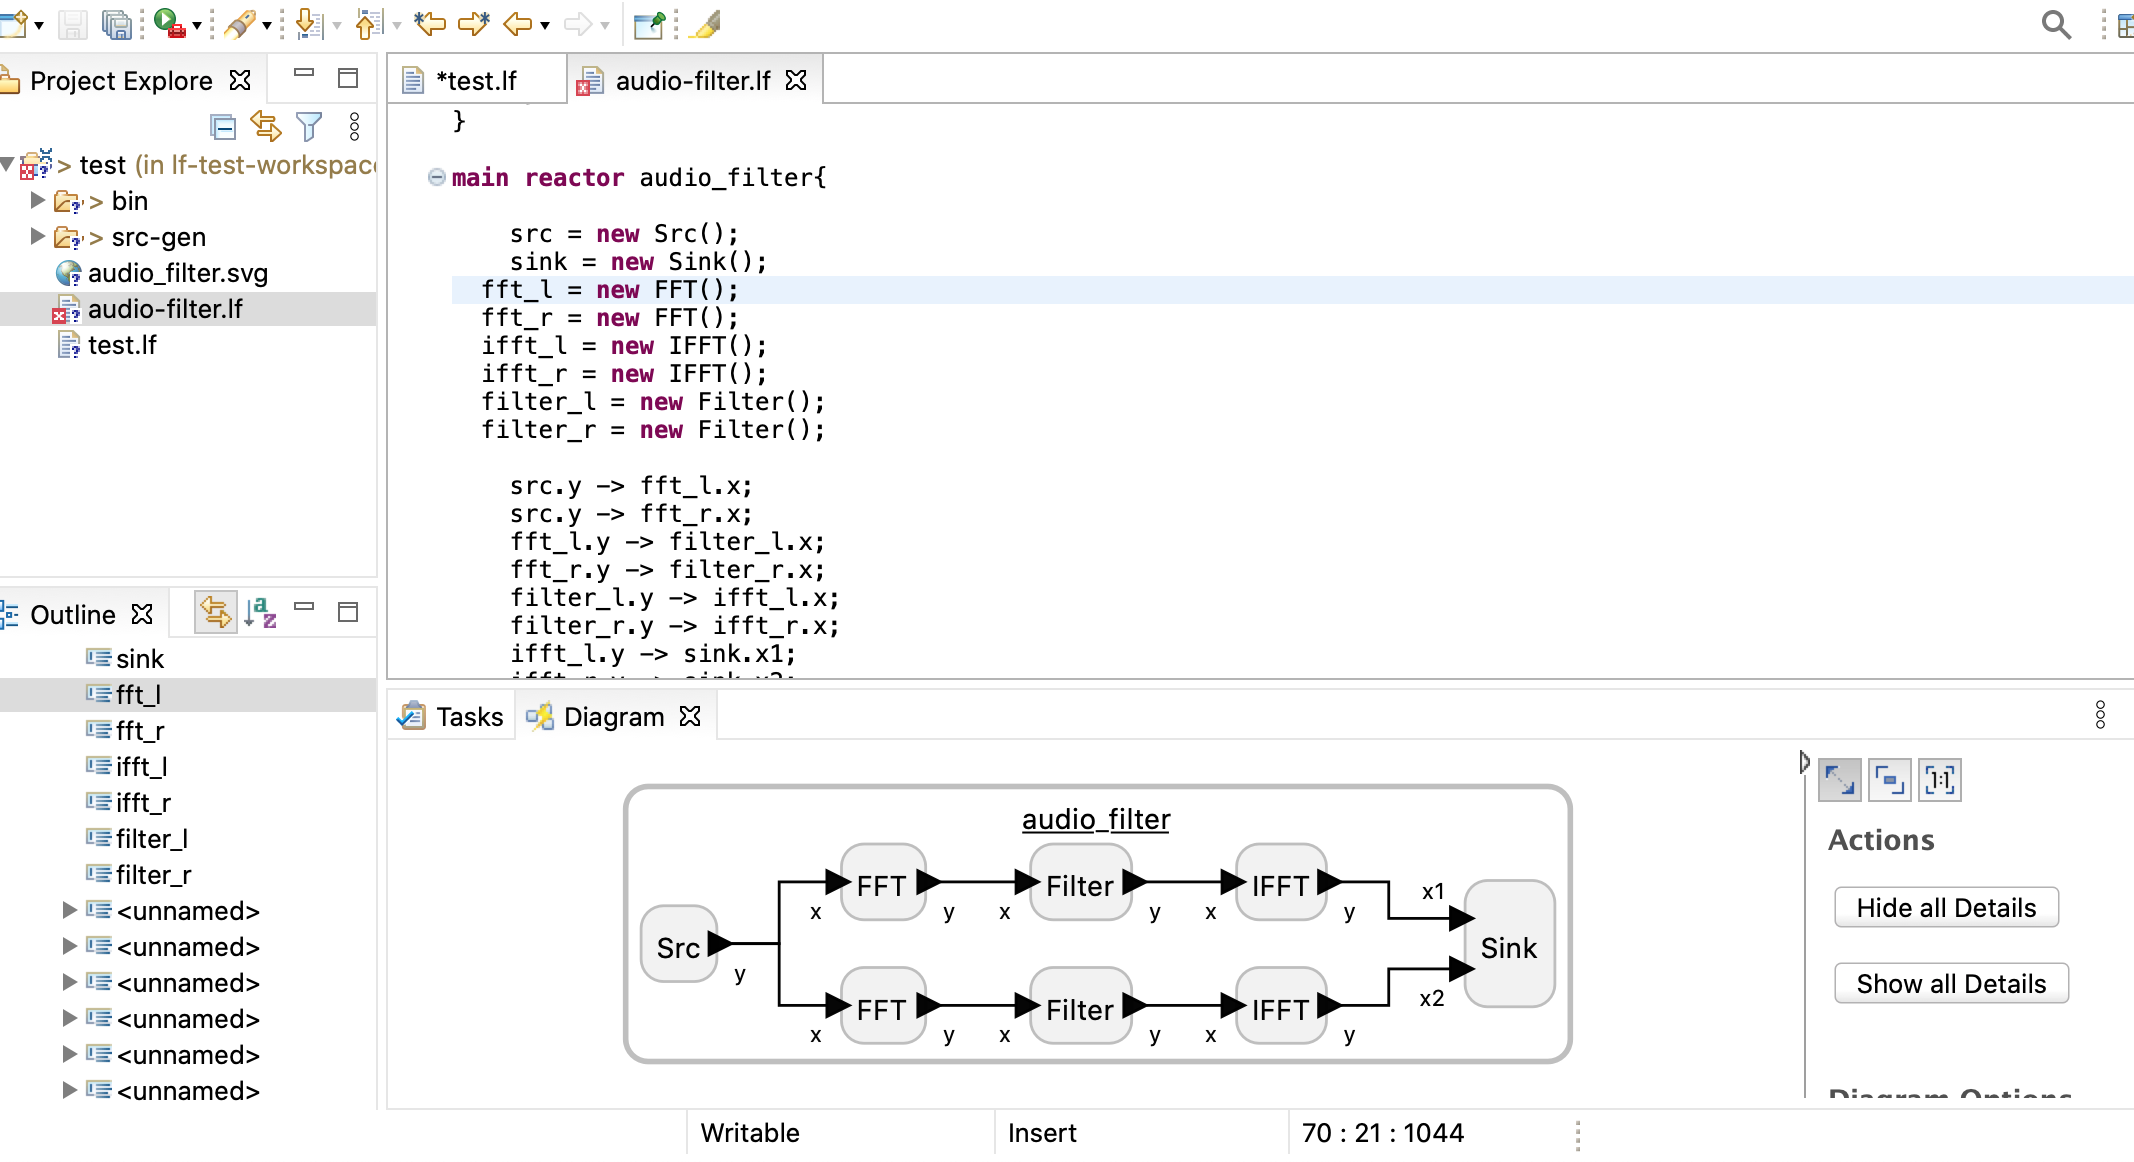
\includegraphics[width=0.9\textwidth]{figures/audio_filter_lf_screenshot.png}
	\caption{The audio filter example in Lingua Franca}
	\label{fig:audio_filter_lf}
	%	\vspace{-1mm}
\end{figure}

In Chapter~\ref{chap:mapping} we discussed the \ac{CPN} language, as well as the \ac{MAPS} framework which is used to lower \ac{CPN} to different implementations in heterogeneous systems.
In contrast\footnote{As an extension of C, the \ac{CPN} language also does not fundamentally prevent programmers from breaking the semantics.}, e.g. the YAPI programming interface~\cite{yapi} defines process networks only as a runtime library and can be evaded just like Scala developers do with actor frameworks~\cite{tasharofi2013scala}.
The Sesame framework uses YAPI-based programs, e.g. derived from Compaan~\cite{stefanov2003deriving} for \ac{DSE}\cite{pimentel2006systematic}.
Most of the software synthesis flows discussed in Section~\ref{sec:software_synthesis_flows} use the languages described here, e.g. TURNUS which uses CAL or SystemCoDesigner which is based on SystemC.
Other systems like DAARM or \mocasin do not use actual source code for the applications but rather application models for \ac{DSE}.


Most of the flows discussed above and in Section~\ref{sec:software_synthesis_flows} are academic and deal with more sophisticated \acp{MoC}. 
Many ideas that seem good in academia do not hold up in a practical development environment, where the learning curve of the models and time-to-market considerations change the field.
It is therefore not surprising that the more sophisticated models have seen less adoption.
Nevertheless, some \ac{MoC}-based commercial systems do exist and have seen successful adoption.
For example, the LabVIEW Communications System Design Suite restricts the LabVIEW language to a dataflow \ac{MoC}.
Similarly, Matlab Simulink has a dataflow-like semantic with time triggering, and is thus closer to discrete event models.
On the discrete events side, as mentioned above, hardware description languages like Verilog or VHDL have discrete-event semantics.
These languages are very widespread and are used commercially.

\subsection{Implicit Dataflow}

The languages surveyed so far are explicit about their abstractions: Actors, Reactors or Processes are declared explicitly.
Similarly, channels describing the data flow are made explicit either through channel declarations or through the connection of explicit ports.
A programmer writing in e.g. \ac{CPN} or Lingua Franca has to have a model of the network describing the application in their head (or in their \acs{IDE}).
Implicit abstractions, on the other hand, work by generating implicit models from linguistic constructs that don't exhibit their structure directly.\index{implicit abstractions}

Implicit abstractions, as we just defined them, are ubiquitous in programming languages.
Objects in \ac{OOP}, for example, are an implicit abstraction for data encapsulation that is fundamentally similar to actors.
A thorough classification  of these implicit models is outside the scope of this thesis.
Instead, we will look closely at the Ohua programming paradigm~\cite{ertel_phdthesis}, which derives a dataflow execution from functional semantics.

The Ohua programming paradigm, by S. Ertel, and others is an implicit model of concurrency. \index{Ohua}
It can  be used to express concurrency at a language level, without explicit constructions, like threads and locks. 
As stated above, the parallelism comes from lowering an Ohua program into a dataflow-based execution.
This model is not part of the original contribution of this thesis.
We will introduce it here as background material.

Ohua itself is a general paradigm that works on multiple languages, and the framework has evolved over the years of its development.
The version of Ohua we will discuss here is based on Clojure and Java, but the Ohua compiler and its principles work with many languages.
Rutimes also exist for Rust, Javascript or Go, at different levels of maturity.
Ohua is best understood by diving directly into examples. 

\begin{listing}
\begin{minted}[linenos]{Clojure}
(defn -main
  "Audio filter example"
  [& args]
  (ohua
   (smap
    (algo [s]
          (let [[x y] (split s)]
            (let [[leftout rightout]
                  [(ifft (filterfn (fft x)))
                   (ifft (filterfn (fft y)))]]
              (sink leftout rightout)
              )
            )
          )
    (src)
    )
   )
  )
\end{minted}
\caption{The Audio Filter Example written in Ohua}
\label{listing:ohua_audio_filter}
\end{listing}

Consider the code in Listing~\ref{listing:ohua_audio_filter}. The code in the example is written in an embedded \ac{DSL} based on Clojure, a dialect of Lisp.
It implements the same example from Chapter~\ref{chap:mapping} (cf. Listing~\ref{listing:audio_filter} or Figure~\ref{fig:audio_filter_graph}), a two-channel audio filter.
Internally, the compiler transforms this code into a dataflow graph for execution.
A special function, \texttt{ohua}, annotates the \ac{AST} it receives as argument to be executed as implicit dataflow.
The \texttt{smap} function is a special variant of \texttt{map} that considers state in the functions.
We will discuss the semantics of \texttt{smap} in Section~\ref{sec:smap}.
Finally, the \texttt{algo} definition in Ohua is akin to the anonymous function definition \texttt{fn} in Clojure.
It defines Ohua ``algorithms'', which are transformed to dataflow actors.
As a \ac{MoC}, this can be embedded in the Dennis dataflow models discussed in Chapter~\ref{chap:mocs}.
%We will discuss the semantics of these dataflow graphs in Section~\ref{sec:ohua_dataflow}.

The example in Listing~\ref{listing:ohua_audio_filter} can be transformed into a dataflow graph for execution.% We will discuss this further in Section~\ref{sec:ohua_dataflow}.
The main advantage of this transformation is that a dataflow graph exposes concurrency, which can be exploited e.g. in a parallel execution or for optimizing \ac{I/O} (cf. Section~\ref{sec:yauhau}).
This duality between code and dataflow graphs is a core concept behind Ohua.
The other central pilar of the Ohua design concept are stateful functions, an abstraction that encapsulates functions with state and side-effects in the context of their dataflow execution.
\index{Ohua ! stateful functions}

\subsection{Stateful Functions}
The functional programming community has made the distinction between \emph{pure} and \emph{impure} functions widespread.
A pure function is a function in the mathematical sense of the word: it receives a certain input and, deterministically, produces an output.
This could be as simple as negating a boolean value, or as complicated as inference with a gargantuan deep neural network.
The main point is that the entirety of the usage of a function is that it returns a value in a deterministic fashion from its inputs.

In most imperative languages, like C or Java, functions usually also have side-effects. Writing the output to the terminal, storing data in a global data structure or even reading data from a sensor in a \ac{CPS}, these are all examples of side effects.
A language that only allows pure functions is basically useless, since even printing the result of a computation is impure.

Stateful functions are a special abstraction, where the concept of pure functions is extended to consider the state of the computation. 
While this excludes aspects like the time of the computation and side-effects like actuation, it is general enough to cover large classes of functions used in most software.
A stateful function is a function $f : a \rightarrow b$ and an abstract state $S$, where the execution of the function can be seen as dependent of the state, which it also modifies.
In other words, we consider $f$ as a function:
\begin{align}
  f : a \times S \rightarrow b \times S \label{eqn:state_thread}
\end{align}

Pure functions can be seen as a special case of stateful functions, with a trivial state $S = \{*\}$.
Listing~\ref{listing:stateful_function} shows an example of a stateful function, written in Java, which is identified as such by the \texttt{@defsfn} annotation~\cite{ertel_pmam18}.
It models a parser, which writes the parsed symbols to a symbol table.
The table, a private object of the class, is the state of this stateful function.
It is implicitly managed as the state by the Ohua runtime.

\begin{listing}
\begin{minted}[]{Java}
public class ParseVariable{
    @defsfn
    private SymbolTable table;
    public ParseVariable (ExpressionObject expr){
        symbols = expr.parse();
        this.table.write(symbols);
        return(this.table.getSymbols());
    }
}
\end{minted}
\caption{An example of a stateful function.}
\label{listing:stateful_function}
\end{listing}